\documentclass[14pt,aspectratio=169]{beamer}

\usepackage{graphicx}
\graphicspath{{figures/}}

\usepackage{booktabs}
\usepackage{tikz}
\usepackage{caption}
\usepackage{xcolor}

\usepackage{subcaption}
\captionsetup[sub]{labelformat=empty}

\usetheme{auriga}
\usecolortheme{auriga}
% \usecolortheme{owl}

% \definecolor{bg-color}{RGB}{25,26,26}
\definecolor{bg-color}{RGB}{255,252,245}
\setbeamercolor{background canvas}{bg=bg-color}

% Remove slide numbers
\setbeamertemplate{footline}{}

\newcommand{\censuscolor}{teal}
\newcommand{\acscolor}{purple}

\makeatletter
\newcommand{\censusVAP}{\@ifnextchar_{\censusVAP@sub}{\censusVAP@nosub}}
\newcommand{\censusVAP@nosub}{{\textcolor{\censuscolor}{\textrm{VAP}}}^{\textcolor{\censuscolor}{\textrm{PL}}}}
\def\censusVAP@sub_#1{{\textcolor{\censuscolor}{\textrm{VAP}}}_{#1}^{\textcolor{\censuscolor}{\textrm{PL}}}}

\newcommand{\acsVAP}{\@ifnextchar_{\acsVAP@sub}{\acsVAP@nosub}}
\newcommand{\acsVAP@nosub}{{\textcolor{\acscolor}{\textrm{VAP}}}^{\textcolor{\acscolor}{\textrm{ACS}}}}
\def\acsVAP@sub_#1{{\textcolor{\acscolor}{\textrm{VAP}}}_{#1}^{\textcolor{\acscolor}{\textrm{ACS}}}}

\newcommand{\acsCVAP}{\@ifnextchar_{\acsCVAP@sub}{\acsCVAP@nosub}}
\newcommand{\acsCVAP@nosub}{{\textcolor{\acscolor}{\textrm{CVAP}}}^{\textcolor{\acscolor}{\textrm{ACS}}}}
\def\acsCVAP@sub_#1{{\textcolor{\acscolor}{\textrm{CVAP}}}_{#1}^{\textcolor{\acscolor}{\textrm{ACS}}}}
\makeatother
\newcommand{\vap}{\textrm{VAP}}
\newcommand{\cvap}{\widehat{\textrm{CVAP}}}

\newcommand{\var}{\mathcal{X}}
\newcommand{\rc}[1]{r_{\textrm{#1}}}

\newcommand{\eqbox}[1]{
    \[
    \tikz[baseline=(eq.base)]{
        \node[
            draw=red!70!black,
            rounded corners,
            line width=1.2pt,
            inner xsep=10pt,
            inner ysep=8pt
        ] (eq) {$\displaystyle #1$};
    }
    \]
}
\newcommand{\eqboxlabel}[2]{
    \[
    \tikz[baseline=(eq.base)]{
        \node[
            draw=red!70!black,
            rounded corners,
            line width=1.2pt,
            inner xsep=10pt,
            inner ysep=8pt,
            label=above:{\footnotesize #2}
        ] (eq) {$\displaystyle #1$};
    }
    \]
}


\title{\normalsize Bayesian Estimation of Block-Level Citizen Voting-Age Population for Redistricting}
\author{\textbf{Christopher Wolfram}, Moon Duchin, Aaron Schein}
\institute[shortinst]{University of Chicago}
% \author{
%     \vspace{0.5cm}
%     \texorpdfstring{
%         \textcolor{gray}{$\underbrace{\text{
%             $\underbrace{
%                 \textcolor{black}{\text{\textbf{Christopher Wolfram}, Moon Duchin}}
%             }_{\text{Department of Computer Science}}$,~
%             $\underbrace{
%                 \textcolor{black}{\text{Aaron Schein}}
%             }_{\text{Department of Statistics}}$
%         }}_{\text{Data Science Institute, University of Chicago}}$}
%     }
%     {Christopher Wolfram, Moon Duchin, Aaron Schein}
% }


\begin{document}


\begin{frame}
    \titlepage
\end{frame}


\begin{frame}{Assessing districting plans}
\centering
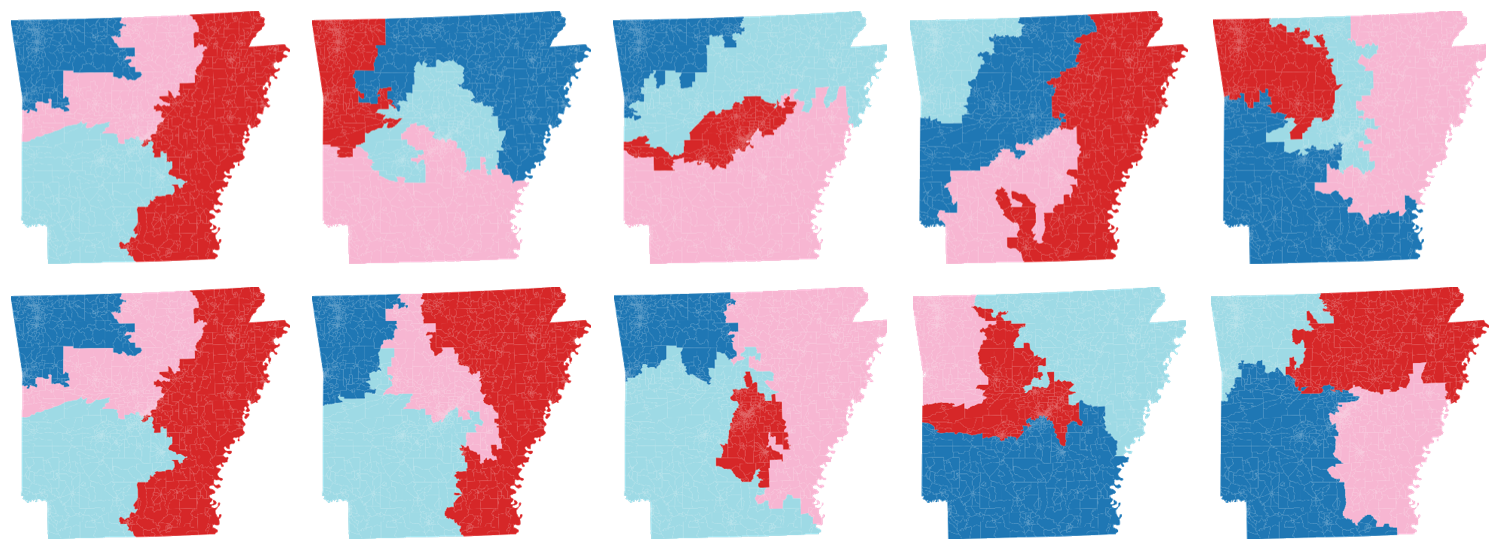
\includegraphics[width=0.8\linewidth]{plans}
\end{frame}


\begin{frame}{CVAP Sources}
\begin{itemize}
    \item Decennial Census?
    \pause
    \begin{itemize}
        \item No \textbf{citizenship} information
    \end{itemize}
    \pause
    \item American Community Survey (ACS)?
    \pause
    \begin{itemize}
        \item Wrong \textbf{spatial resolution}
        \pause
        \item Wrong \textbf{race/ethnicity categories}
    \end{itemize}
\end{itemize}
\end{frame}


% \begin{frame}{The Trouble with CVAP}
% \begin{enumerate}
%     \item Citizenship data is only availible at a \textbf{lower spatial resolution} than is needed
%     \vspace{0.5cm}
%     \pause
%     \item The \textbf{race/ethnicity categories} for which citizenship data is availible are different from those which are relevant for litigation
% \end{enumerate}
% \end{frame}

% \begin{frame}{The Trouble with CVAP}
% \begin{enumerate}
%     \item \textbf{Spatial resolution}
%     \vspace{0.5cm}
%     \pause
%     \item \textbf{Race/ethnicity categories} for litigation
% \end{enumerate}
% \end{frame}



\begin{frame}
    \centering
    {\LARGE \bf Spatial Resolution \& \\ \bigskip Small Area Estimation}
\end{frame}


% \begin{frame}{Redistricting Geography}
% \centering
% 
\includegraphics[width=0.8\linewidth]{baseMap.pdf}
% \end{frame}


\begin{frame}{Redistricting Geography}
\centering
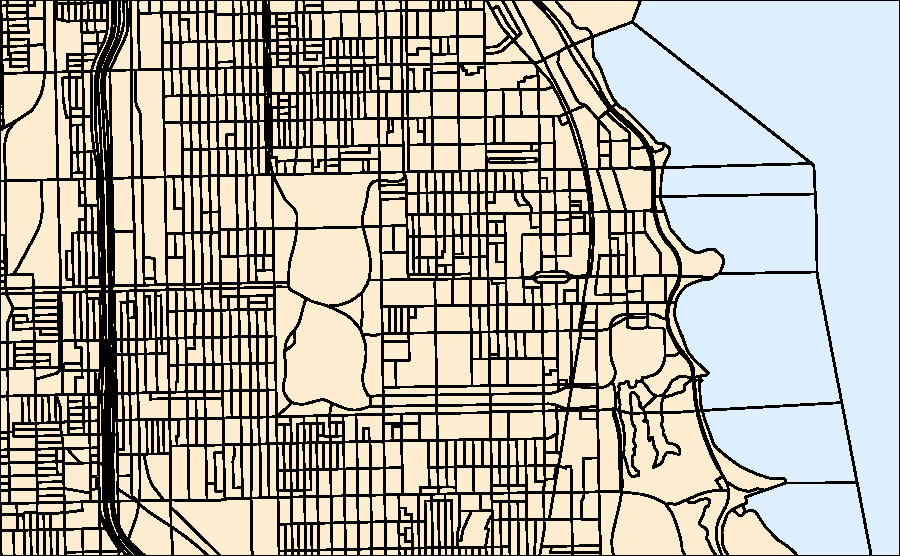
\includegraphics[width=0.8\linewidth]{blockMap.pdf}
\end{frame}


\begin{frame}{Redistricting Geography}
\centering
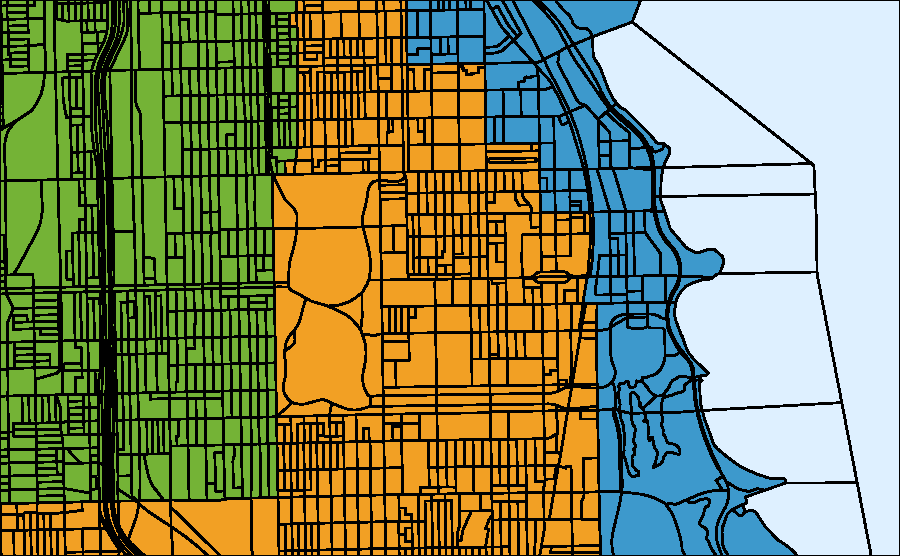
\includegraphics[width=0.8\linewidth]{blockDistrictMap.pdf}
\end{frame}


\begin{frame}{Redistricting Geography}
\centering
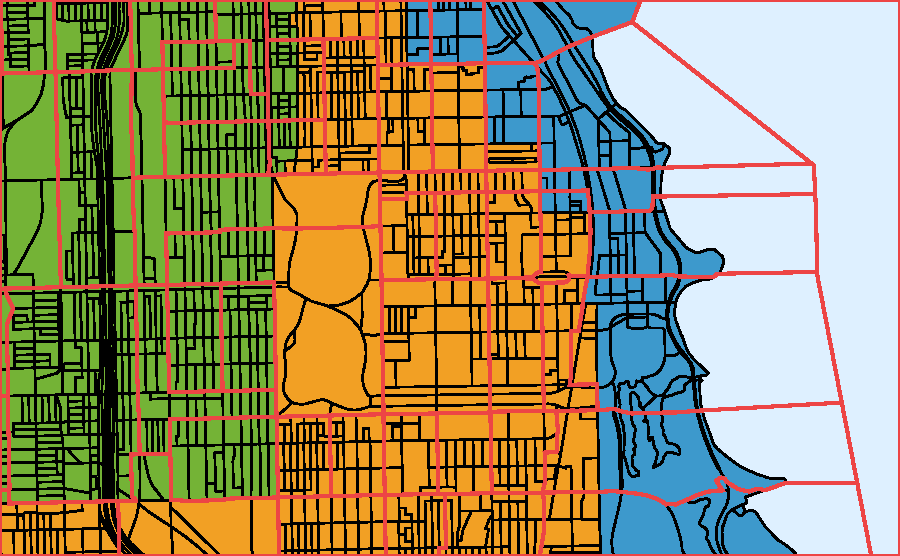
\includegraphics[width=0.8\linewidth]{blockTractDistrictMap.pdf}
\end{frame}


\begin{frame}{Redistricting Geography}
\centering
\begin{tikzpicture}
    \node[inner sep=0] (img) {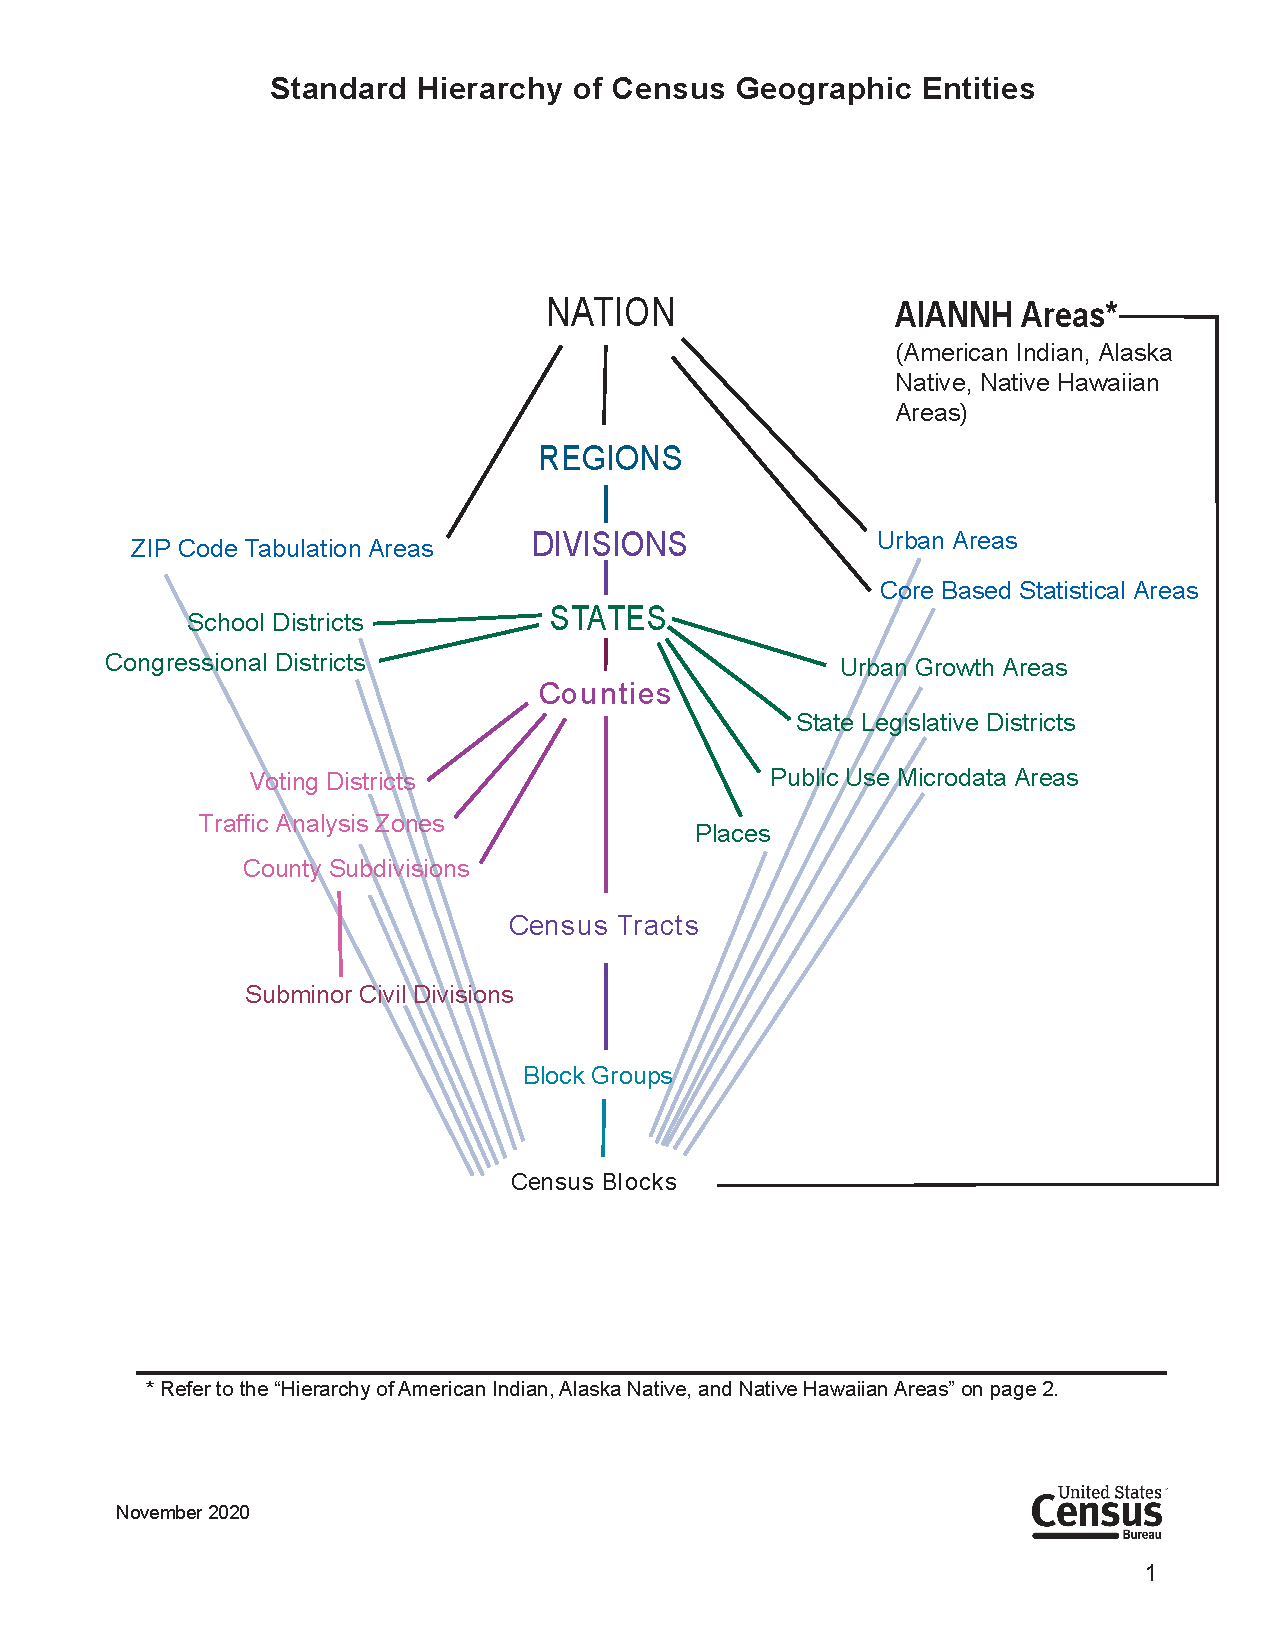
\includegraphics[width=0.6\linewidth, page=1, trim=0.9cm 7cm 0.9cm 5cm, clip]{geodiagram.pdf}};
    \pause
    \begin{scope}[shift={(img.south west)}, x={(img.south east)}, y={(img.north west)}]
        \draw[red, line width=2pt] (0.165, 0.61) ellipse [x radius=0.15, y radius=0.05];
    \end{scope}
\end{tikzpicture}
\end{frame}


\begin{frame}{Observed Variables}
    \centering
    $\underbrace{\censusVAP}_{\text{block-level}}$ \hspace{1cm} $\underbrace{\acsVAP, \acsCVAP}_{\text{tract-level}}$
\end{frame}


\begin{frame}{Dissaggregation}
    $$\cvap_b = \acsCVAP_{t[b]} \times \frac{\text{CVAP in $b$}}{\text{CVAP in $t[b]$}}$$
    \pause
    \vspace{0.3cm}
    $$\frac{\censusVAP_b}{\censusVAP_{t[b]}} \approx \frac{\text{CVAP in $b$}}{\text{CVAP in $t[b]$}}$$
    \pause
    \vspace{0.3cm}
    \eqboxlabel{\cvap_b \approx \acsCVAP_{t[b]} \times \frac{\censusVAP_b}{\censusVAP_{t[b]}}}{Dissaggregation formula}
\end{frame}


\begin{frame}{Dissaggregation's assumption}
    $$\cvap_b \approx \acsCVAP_{t[b]} \times \frac{\censusVAP_b}{\censusVAP_{t[b]}}$$
    \pause
    \vspace{0.3cm}
    \eqboxlabel{\frac{\cvap_b}{\acsCVAP_{t[b]}} \approx \frac{\censusVAP_b}{\censusVAP_{t[b]}}}{Dissaggregation assumption}
\end{frame}


\begin{frame}{Discounting}
    $$\cvap_b \approx \censusVAP_b \times \underbrace{\frac{\acsCVAP_{t[b]}}{\acsVAP_{t[b]}}}_{\textrm{citizenship rate}}$$
    \pause
    \vspace{0.3cm}
    \eqboxlabel{\frac{\cvap_b}{\censusVAP_b} \approx \frac{\acsCVAP_{t[b]}}{\acsVAP_{t[b]}}}{Discounting assumption}
\end{frame}


\begin{frame}{Dissaggregation vs. Discounting}
    \eqboxlabel{\frac{\cvap_b}{\acsCVAP_{t[b]}} \approx \frac{\censusVAP_b}{\censusVAP_{t[b]}}}{Dissaggregation assumption}

    \eqboxlabel{\frac{\cvap_b}{\censusVAP_b} \approx \frac{\acsCVAP_{t[b]}}{\acsVAP_{t[b]}}}{Discounting assumption}
\end{frame}


\begin{frame}{Practical Problem with Discounting}
    \centering
    $$\cvap_b \approx \censusVAP_b \times \underbrace{\frac{\acsCVAP_{t[b]}}{\acsVAP_{t[b]}}}_{\textrm{citizenship rate}}$$

    \vspace{0.5cm}
    \pause

    What if $\acsVAP_{t[b]} = 0$?
    \pause

    \medskip

    What if $\acsVAP_{t[b]}$ is just small?
\end{frame}


\begin{frame}{Why is this not a problem for Dissaggregation?}
    It is! It's not a numerical problem, but it is a statistical problem.
\end{frame}


\begin{frame}{Bayesian Discounting}
    \begin{align*}
        \omega_{t[b]} &\sim \textrm{Beta}(\alpha, \beta) \\
        \acsCVAP_{t[b]} &\sim \textrm{Binomial}(\acsVAP_{t[b]}, \omega_{t[b]}) \\
        \cvap_b &\sim \textrm{Binomial}(\censusVAP_b, \omega_{t[b]})
    \end{align*}

    \vspace{0.5cm}
    \pause

    \centering
    \begin{minipage}{0.6\textwidth}
        \begin{itemize}
            \setlength{\itemsep}{0.2em}
            \item Discrete support!
            \pause
            \item Uncertainty quantification!
            \pause
            \item No numerical problems!
        \end{itemize}
    \end{minipage}
\end{frame}


\begin{frame}{Beta-Binomial Conjugacy}
    Prior and likelihood:
    \begin{align*}
        \omega_{t[b]} &\sim \textrm{Beta}(\alpha, \beta) \\
        \acsCVAP_{t[b]} &\sim \textrm{Binomial}(\acsVAP_{t[b]}, \omega_{t[b]})
    \end{align*}

    \pause

    Posterior:
    $$\omega_{t[b]} \mid - \sim \textrm{Beta}\!\left(\alpha + \acsCVAP_{t[b]},\ \beta + \acsVAP_{t[b]} - \acsCVAP_{t[b]}\right)$$

    \pause

    Posterior mean:
    $$\hat{\omega}_{t[b]} = \frac{\alpha + \acsCVAP_{t[b]}}{\alpha + \beta + \acsVAP_{t[b]}} \pause \approx \underbrace{\frac{\acsCVAP_{t[b]}}{\acsVAP_{t[b]}}}_{\text{naive estimator}}$$
\end{frame}


\begin{frame}{Fitting the Bayesian Discounting Model}
    Citizenship rate prior:
    \begin{equation*}
        \omega_{t[b]} \sim \textrm{Beta}(\alpha, \beta), \hspace{0.5em} \alpha \approx 0.84, \hspace{0.5em} \beta \approx 0.29
    \end{equation*}

    \centering
    \only<1>{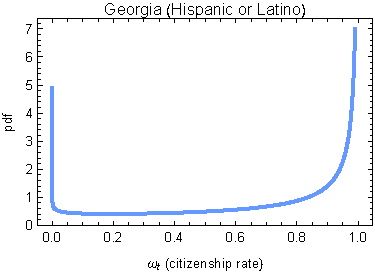
\includegraphics[width=0.5\linewidth]{empDist0.pdf}}
    \only<2>{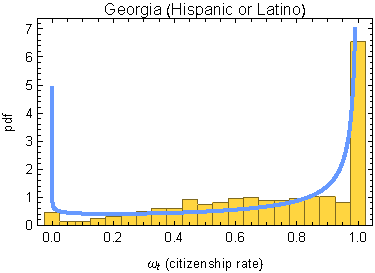
\includegraphics[width=0.5\linewidth]{empDist2.pdf}}
    \only<3>{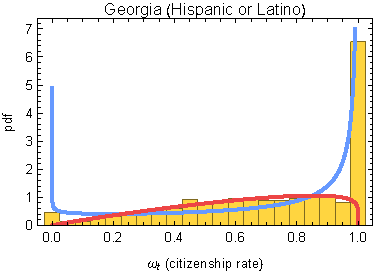
\includegraphics[width=0.5\linewidth]{empDist3.pdf}}
\end{frame}

\begin{frame}{It is not just tiny tracts}
    \centering
    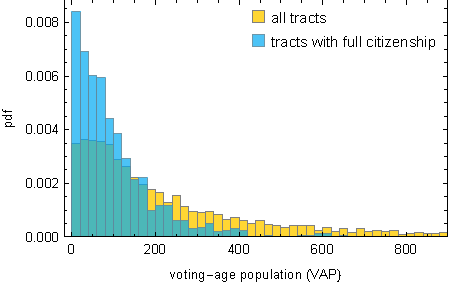
\includegraphics[width=0.7\linewidth]{citizenship_pop_hists.pdf}
\end{frame}


% \begin{frame}{Uncertainty in $\acsCVAP$ \& $\acsVAP$}
% \end{frame}


\begin{frame}{Bonus: Bayesian Dissaggregation}
    \begin{align*}
        \omega_b &\sim \textrm{Beta}(\alpha, \beta) \\
        \censusVAP_b &\sim \textrm{Binomial}(\censusVAP_{t[b]}, \omega_b) \\
        \cvap_b &\sim \textrm{Binomial}(\acsCVAP_{t[b]}, \omega_b)
    \end{align*}
\end{frame}


\begin{frame}
    \centering
    {\LARGE \textbf{Race/Ethnicity Categories}}
\end{frame}


\begin{frame}{Challenges}
    \begin{itemize}
        \item The race/ethnicity categories used for ACS CVAP are not those relevant for litigation.
        \item The ACS race question differed from the Decennial Census question until 2020.
    \end{itemize}
\end{frame}


\begin{frame}{Census Questionaire}
    \centering
    \includegraphics[width=0.35\textwidth, page=3, trim={1.7cm 1.1cm 11.4cm 21.3cm}, clip]{questionaires/2020-informational-questionnaire-english_DI-Q1.pdf}
    \hspace{0.5cm}
    \includegraphics[width=0.35\textwidth, page=3, trim={12cm 12.5cm 1cm 1cm}, clip]{questionaires/2020-informational-questionnaire-english_DI-Q1.pdf}
\end{frame}


\begin{frame}{ACS Detailed Tables Race/Ethnicity Categories}
    \centering
    \begin{itemize}
        \setlength\itemsep{0em}
        \item White Alone
        \item Black or African American Alone
        \item American Indian and Alaska Native Alone
        \item Asian Alone
        \item Native Hawaiian and Other Pacific Islander Alone
        \item Some Other Race Alone
        \item Two or More Races
        \item Hispanic or Latino
        \item White Alone, Not Hispanic or Latino
        \item Total
      \end{itemize}
\end{frame}



\begin{frame}{}
    Let $\var_{g,h,\rc{W},\rc{B},\ldots,\rc{O}}$ be the count of people in geography $g$ with Hispanic or Latino ethnicity $h$ and race categories $\rc{W},\rc{B},\ldots,\rc{O}$

    \bigskip\pause

    For example, $$\var_{g=1029, h=1, \rc{W}=0, \rc{B}=0, \rc{A}=1, \dots, \rc{O}=1} = 21$$

    \bigskip\pause

    $$\var \in \mathbb{Z}_+^{|G| \times 2 \times 2 \cdots}$$
\end{frame}


\begin{frame}
    \scriptsize
    \begin{align*}
        \var_{g,\rc{W}=1} &= \sum_{h \in \{0,1\}} \var_{g,h,\rc{W}=1, \rc{B}=0, \dots, \rc{O}=0} \tag{White Alone} \\
        \var_{g,\rc{B}=1} &= \sum_{h \in \{0,1\}} \var_{g,h,\rc{W}=0, \rc{B}=1, \dots, \rc{O}=0} \tag{Black or African American Alone} \\
        \vdots \\
        \var_{g,2+} &= \sum_{h,\rc{W},\rc{B},\dots,\rc{O} \in \{0,1\}} \mathbf{1}(\rc{W} + \rc{B} + \dots + \rc{O} \geq 2)\var_{g,h,\rc{W}, \rc{B}, \dots, \rc{O}} \tag{Two or More} \\
        \var_{g,h=1} &= \sum_{\rc{W},\rc{B},\ldots,\rc{O} \in \{0,1\}} \var_{g,h=1,\rc{W},\rc{B},\ldots,\rc{O}} \tag{Hispanic or Latino} \\
        \var_{g,h=0,\rc{W}=1} &= \var_{g,h=0,\rc{W}=1,\rc{B}=0,\ldots,\rc{O}=0} \tag{White Alone, Not Hispanic or Latino} \\
        \var_{g} &= \sum_{h,\rc{W},\rc{B},\dots,\rc{O} \in \{0,1\}} \var_{g,h,\rc{W}, \rc{B}, \dots, \rc{O}} \tag{Overall} \\
        \var_{g,h,\rc{W}=0,\rc{B}=0,\ldots,\rc{O}=0} &= 0 \tag{No race selected} \\
        \var_{g^\star,h,\rc{W},\rc{B},\dots,\rc{O}} &= \sum_{g \in g^\star} \var_{g,h,\rc{W}, \rc{B}, \dots, \rc{O}} \tag{PUMS}
    \end{align*}
\end{frame}


\begin{frame}{Equivalent Formulation}
    Let $x \in \mathbb{Z}_+^n$ be a flattened version of $\var$.

    \bigskip\pause

    Let $S_j$ be a set of indices of $x$ included in the $j$th available marginal.

    \bigskip\pause

    Let $\displaystyle y_j = \sum_{i \in S_j} x_i$ be the $j$th marginal and $\tilde{y}_j = y_j + \epsilon_j$.

    \bigskip\pause

    \textbf{The problem}: We observe $\tilde{y}$ and $S_j$ and want to recover $x$.
\end{frame}


\begin{frame}{Least Squares Formulation}
    $$y_j = \sum_{i \in S_j} x_i$$

    \medskip\pause

    \begin{align*}
        A_{j,i} &= \mathbf{1}\{i \in S_j\} \\
        y &= Ax % \\
        % \mathcal{F}(y) &= \{x \in \mathbb{Z}_+^n : Ax = y\}
    \end{align*}

    \medskip\pause

    \centering
    Minimize $\|Ax - \tilde{y}\|_2^2$ subject to $x \in \mathbb{Z}_+^n$
\end{frame}


\begin{frame}{Poisson-Poisson Model}
    \begin{align*}
        x_i &\sim \mathrm{Poisson}(\lambda_i) \\
        \tilde{y}_j &\sim \mathrm{Poisson}\bigg (\sum_{i \in S_j} \lambda_i\bigg )
    \end{align*}
\end{frame}


\begin{frame}{ACS vs. Decennial Census Differences}
    \centering
    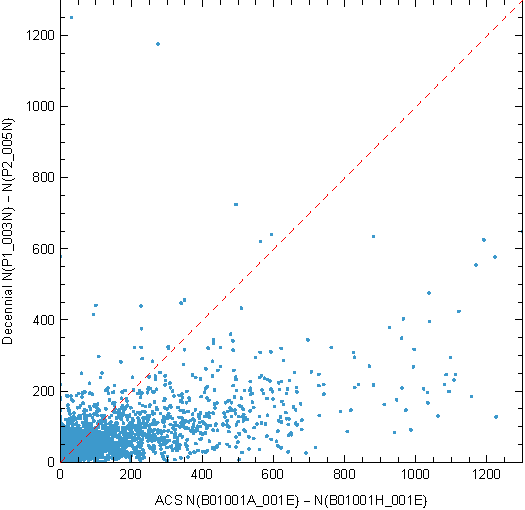
\includegraphics[width=0.5\linewidth]{tract_ACS_dec_alignment.pdf}
\end{frame}


\begin{frame}{ACS vs. Decennial Census Differences}
    \centering
    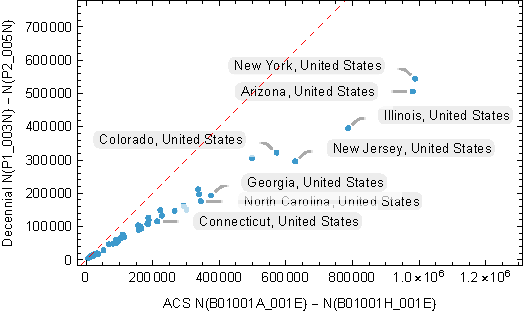
\includegraphics[width=0.7\linewidth]{state_ACS_dec_alignment.pdf}
\end{frame}


\begin{frame}{Questionaire Changes}
    \begin{figure}[t]
        \centering
        \begin{subfigure}[b]{0.32\textwidth}
            \includegraphics[width=\textwidth, page=3, trim={12cm 12.5cm 1cm 1cm}, clip]{questionaires/2020-informational-questionnaire-english_DI-Q1.pdf}
            \caption{2020 Decennial Census}
        \end{subfigure}
        \hfill
        \begin{subfigure}[b]{0.29\textwidth}
            \includegraphics[width=\textwidth, page=2, trim={10.5cm 4cm 1.7cm 8.75cm}, clip]{questionaires/quest20.pdf}
            \caption{2020 ACS}
        \end{subfigure}
        \hfill
        \begin{subfigure}[b]{0.32\textwidth}
            \includegraphics[width=\textwidth, page=2, trim={0.75cm 0.95cm 13.15cm 17.3cm}, clip]{questionaires/quest19.pdf}
            \caption{2019 ACS}
        \end{subfigure}
    \end{figure}
\end{frame}


\begin{frame}{ACS vs. Decennial Census Differences}
    \centering
    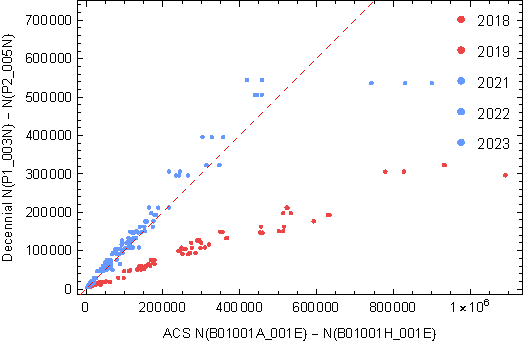
\includegraphics[width=0.7\linewidth]{state_1year_ACS_dec_alignment.pdf}
\end{frame}


\end{document}
